\section{Chapter 9: Images, Narrative, Gestures for explanation}
\graphicspath{ {pngs/ch9/} }


\secttoc

Most complex visualizations involve visual and verbal material.
Exploration, and now a narrative explanation of patterns, have been covered.
It is important to make cross-references and use the most appropriate medium.
Deictic gestures are the most elementary and fundamental.

\begin{mdframed}\begin{multicols}{2}
\subsection{The Nature of Language}
\begin{compactdesc}
\item[Chomsky's Deep Structures] are linguistic featrues that represent innate
    cognitive abilities based on neural structures.
\item[Sign Language] truly visual languages, always with the same complexity as
    spoken language. Many signs are fully abstract. Language has distinct brain
    subsytems, activated no matter the medium.
\item[Dynamic and Linear] speech, signing, even text are understood as streams
    of utterances; unlike static pictures which can be understood in parallel.
\item[Visual Programming] static diagram system: like learning a new language.
    Logical constructs are not typically expressed visually, thus it is
    best to use serial languages for programming.
\item[Images, Sentences, Paragraphs] Language: elaborate, complete and widely
    shared. Images should only be used when necessary. It takes time to
    process a complex diagram, simple line drawings are fastest to comprehend.
\item[Links between Images and Words] theory: it is critical that visual and
    verbal systems be actively constructed, along with interconnections.
    Images and words in unison are more effective than either in isolation.
    Must choose appropriate presentations.
\end{compactdesc}

\begin{figure}[H]\centering
    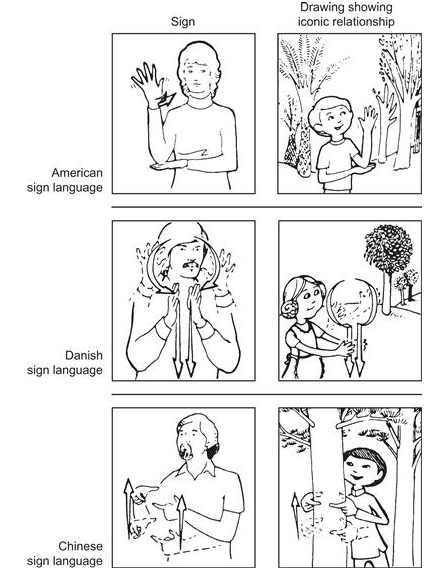
\includegraphics[width=0.65\linewidth]{sign_language.png}
    \caption{Three sign language representations of a tree. All very different.}
\end{figure}

\end{multicols}\end{mdframed}



\begin{mdframed}\begin{multicols}{2}
\subsection{Integrating Visual and Verbal and the Narrative Thread}
\begin{compactdesc}
\item[Linking Text with Graphical Elements] text labels. Also, integrated
    blocks of text help us retain the information, augment the verbal
    system's limited memory. Text and figures are typically separated in
    textbooks -- a decline in cognitive efficiency.
\item[Gestures as Linking Devices] in verbal presentations. Impossible to look
    at a diagram and read text, but one can look and listen to a verbal
    narrative.
\item[Deixis] a pointing gesture. Typically used to indicate subject or
    object in a sentence. Rich vocabulary: can indicate a group of objects,
    or uncertainty in a region. Web-site: highlighting the image or elements a
    sentence refers to increases understanding.
    Help bridge the gap between imagery and speech.
\item[Symbolic Gestures] raised hand = stop, wave hand = hello\dots Some
    gestures represent actions, rotate hand = rotate object, these are called
    kinetographics. tech like Microsoft Kinect make this affordable, but it is
    still experimental.
\item[Expressive Gestures] hand motion called a \textsl{beat} = critical
    element in narrative. Vigorous gestures = vocal stress.
\end{compactdesc}

\subsection{Animated versus Static Presentations}
Animated presentations were once claimed to be superior to static presentations.
This is false. Animated demonstrations help with short term mimicry; but
written explanations, though slower, result in long-term understanding.

This may be because animation hides previous and future images. A static
sequence diagram lets the user perform the animation mentally, and only when
needed. Thus they are superior.

\begin{figure}[H]\centering
    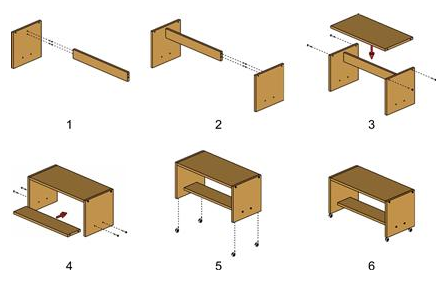
\includegraphics[width=0.8\linewidth]{assembly_diagram.png}
    \caption{Assembly diagram, employs good design principles}
\end{figure}
\end{multicols}\end{mdframed}


\begin{mdframed}\begin{multicols}{2}
\subsection{Visual Narrative}
\begin{compactdesc}
\item[Visual narrative] can be constructed by linear exposition of objects,
    by camera movements and scene transitions. Like silent movies.
\item[Overview then detail] produces more reliable identification than the
    reverse order.
\item[Anchor] a visual reference point. Help link one view of data with the
    next.
\item[Animated images] best if short, otherwise much time must be spent scanning
    a large animation for a static detail. Hitting, pushing, aggression and
    most importantly causality can be expressed using dynamic, but not static
    displays.
\item[Mirror neurons] people learn perceptual motor tasks and skills, even
    become more motivated by imitating others' motions.
\end{compactdesc}

\end{multicols}\end{mdframed}




